\chapter{Literature Review} % Main chapter title

\label{Chapter2} % For referencing this chapter elsewhere, use \ref{Chapter2}

\lhead{Chapter 2. \emph{Literature Review}}

%----------------------------------------------------------------------------------------
%	SECTION 1 - Background - Number representation
%----------------------------------------------------------------------------------------

\section{Background: On number representation}

The question of the representation of numbers as we, humans, use them in a world of electronics has been central in the creation of computers and their associated arithmetics. Several problems are contained in the simple question of: How to translate our arithmetic and number operations in a piece of hardware?

%-----------------------------------
%	SUBSECTION 1 - Number Representation
%-----------------------------------
\subsection{Number Representation}

The first thing to note is that electronics can represent two states, a presence or absence of an electric impulsion. The states of \guille{on} and \guille{off} is embedded in transistors that can represent both. The transistor is the hardware representant of this duality while a bit is its software counter-part. This is the underlying reason why computers, even the first fully electronical computer ENIAC (\emph{Electronical Numerical Integrator and Computer}), use a binary system. If this system is handy to translate our base 10 arithmetic and simple numbers such as integers, it is harder to translate more complex numbers such as reals and floating point operations. The meaning of an N-bit binary word is entirely dependent of the interpretation we choose to use. This interpretation consists of both a representation (the type of the object the memory represents) as well as its associated mapping. Common number representations consists of unsigned integers, signed integers (using two's complement), floating point reals as well as fixed-point reals.

%-----------------------------------
%	SUBSUBSECTION 1 - Integer Representation
%-----------------------------------
\subsubsection{Integer Representation}

The representation of integers and especially unsigned integers is straightforward as it consists of a change form base 10 to base 2. This number representation can be done in 16-bits, 32-bits or 64-bits depending on its type, the supporting hardware and the space we need to contain it. Representing a number in base 2 from base 10 or vice versa is straightforward as it only demands simple and exact basic operations to be performed.

Now, if we want to represent a signed integer, we have to use a method called the two's complement in order to bring the sign in. This method keeps the basic behaviour of the addition to work on numbers be they positive or negative. The method consists in changing the value of all the bits of a given number then adding one to the result.

\begin{figure}[htbp]
	\centering
		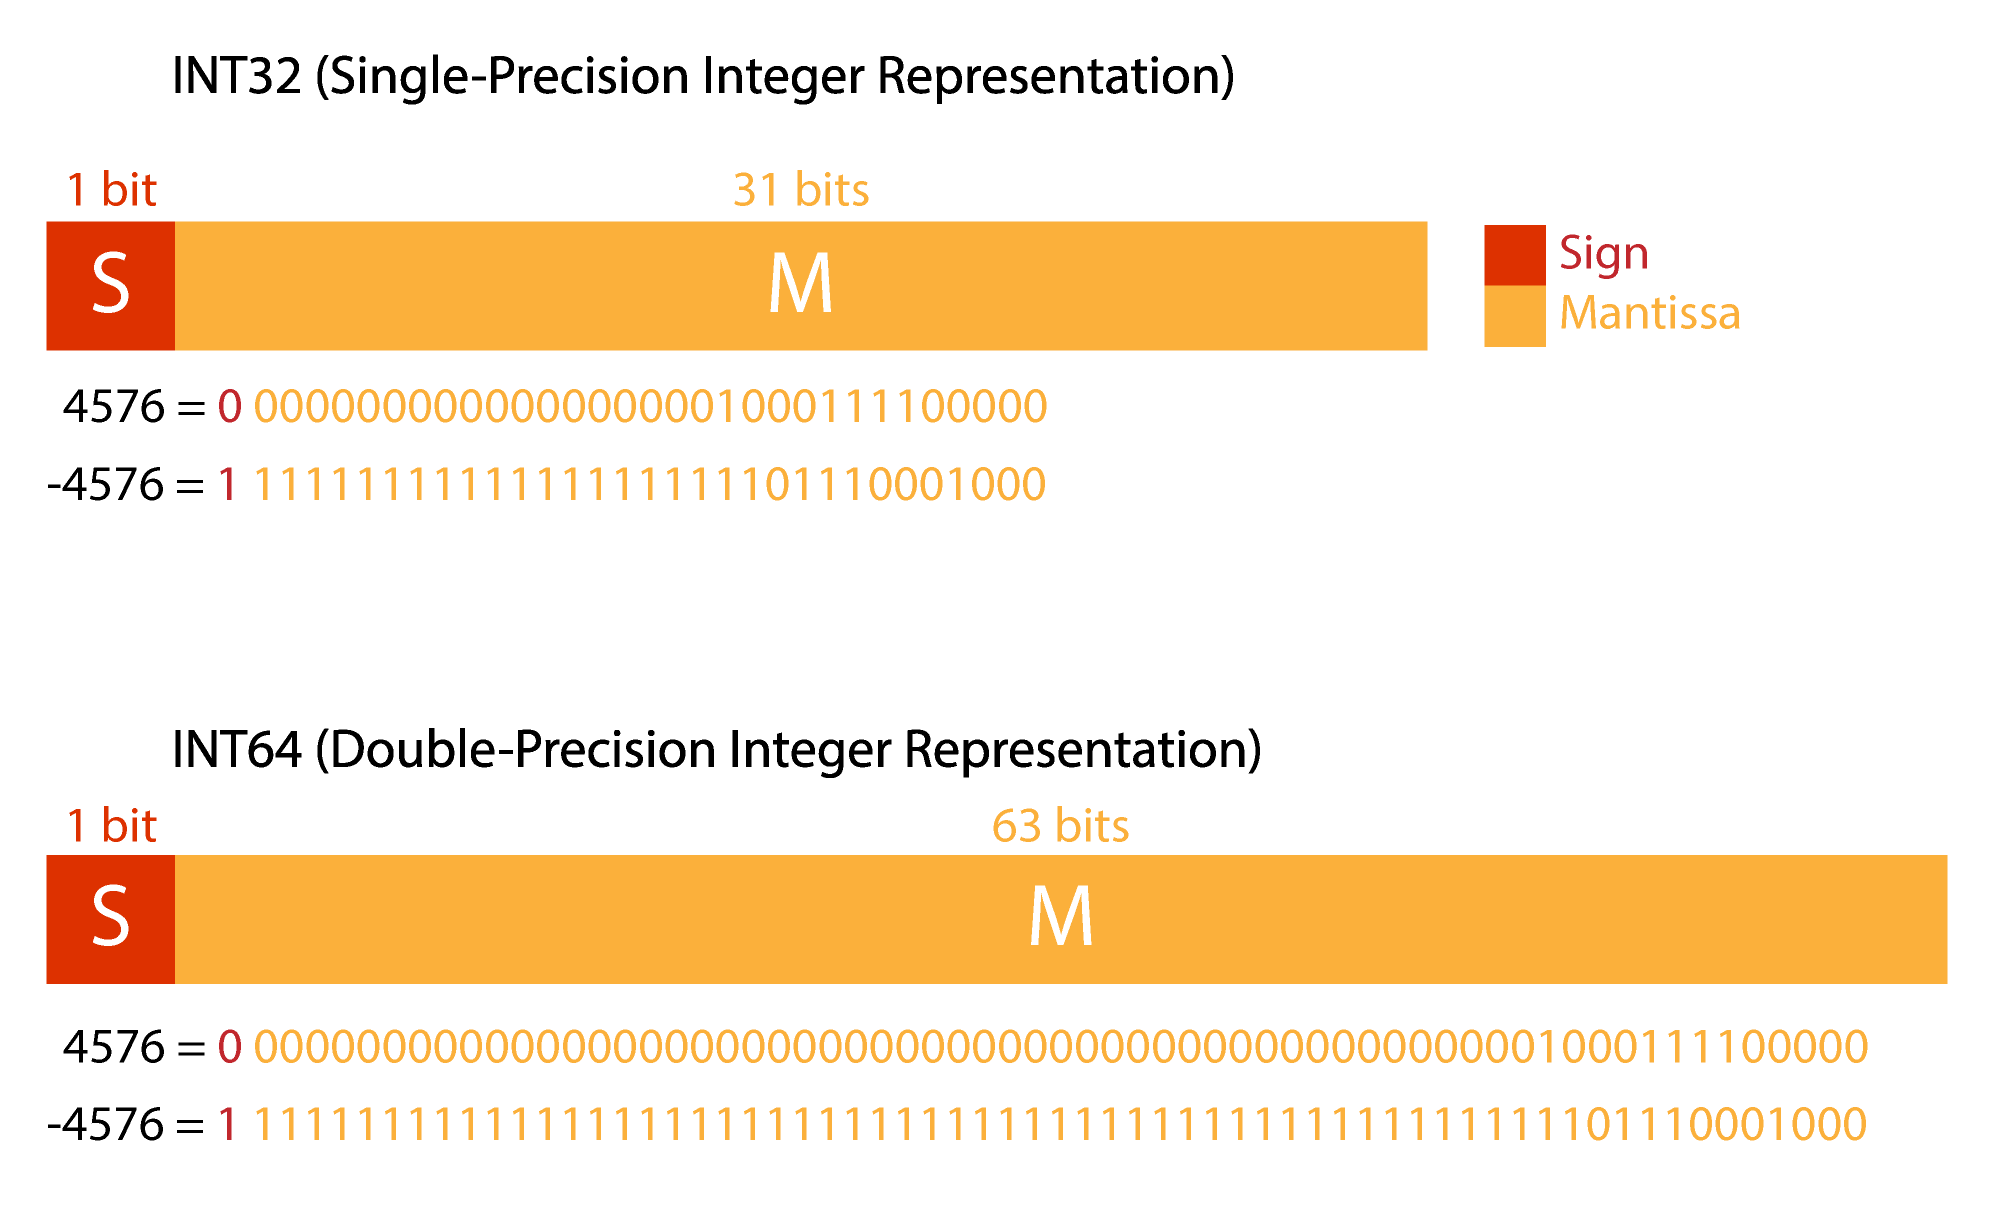
\includegraphics[width=.8\textwidth]{Figures/IntegerRepr.png}
	\caption[Integer Representation]{Integer Representation and Two's Complement example}
	\label{fig:IntegerRepr}
\end{figure}

Those two representations allow a complete mapping of integers up to a certain range: signed 32-bit integers can represent base 10 numbers between -2,147,483,648 and 2,147,483,647 while unsigned integers can represent base 10 numbers between 0 and 4,294,967,295.

%-----------------------------------
%	SUBSUBSECTION 2 - Floating-Point Representation
%-----------------------------------
\subsubsection{Floating-Point Representation}

Representing floating-point numbers has been a concern since the 1980's and the industrial development of several computing modules and interfaces. The need for a consensus in this domain and particular applications has been answered by the IEEE-754 standard \cite{Ieee754_1985} in 1985. This standard defines both the floating-point number representations and exceptions conditions along with their default handling. This norm was reviewed fundamentally in 2008 \cite{Ieee754_2008}, extending it to 64-bits and 128-bits length. The last dated revision of the norm is from 2019 \cite{Ieee754_2019}.

Floating-point numbers following this representation are composed of three distinct elements:
\begin{enumerate}
  \item A sign bit
  \item An exponent
  \item A mantissa
\end{enumerate}

Those three elements compose the number by using the following formula:
\begin{equation}
  (sign) \times mantissa \times 2^{exponent}
\end{equation}

In order to present both positive and negative exponents and as using the two's complement on the exponent would complexify the computation of floating-point numbers, a bias is used in the exponent. This bias corresponds to $2^e - 1$ where e is the number of bits of the exponent part. This means that with an 8-bit exponent, the bias is equal to 127. An exponent equal to $00000111$ is equal to $7 - 127 = -120$ and an exponent equal to $10000111$ is equal to $135 - 127 = 8$. An 8-bit exponent can cover a range from -126 to 127 (because exponents -127 (all 0s) and +128 (all 1s) are reserved for special numbers.

When referring to single-precision floating-point representation we are talking about 32-bit long memory representation. They are mapped as follows and as shown in \emph{Figure} \ref{fig:FP32}:
\begin{itemize}
  \item Sign bit: 1 bit
  \item Exponent: 8 bits
  \item Mantissa: 23 bits
  \item Exponent Bias: 127
\end{itemize}

% FP32 EXAMPLE
\begin{figure}[htbp]
	\centering
		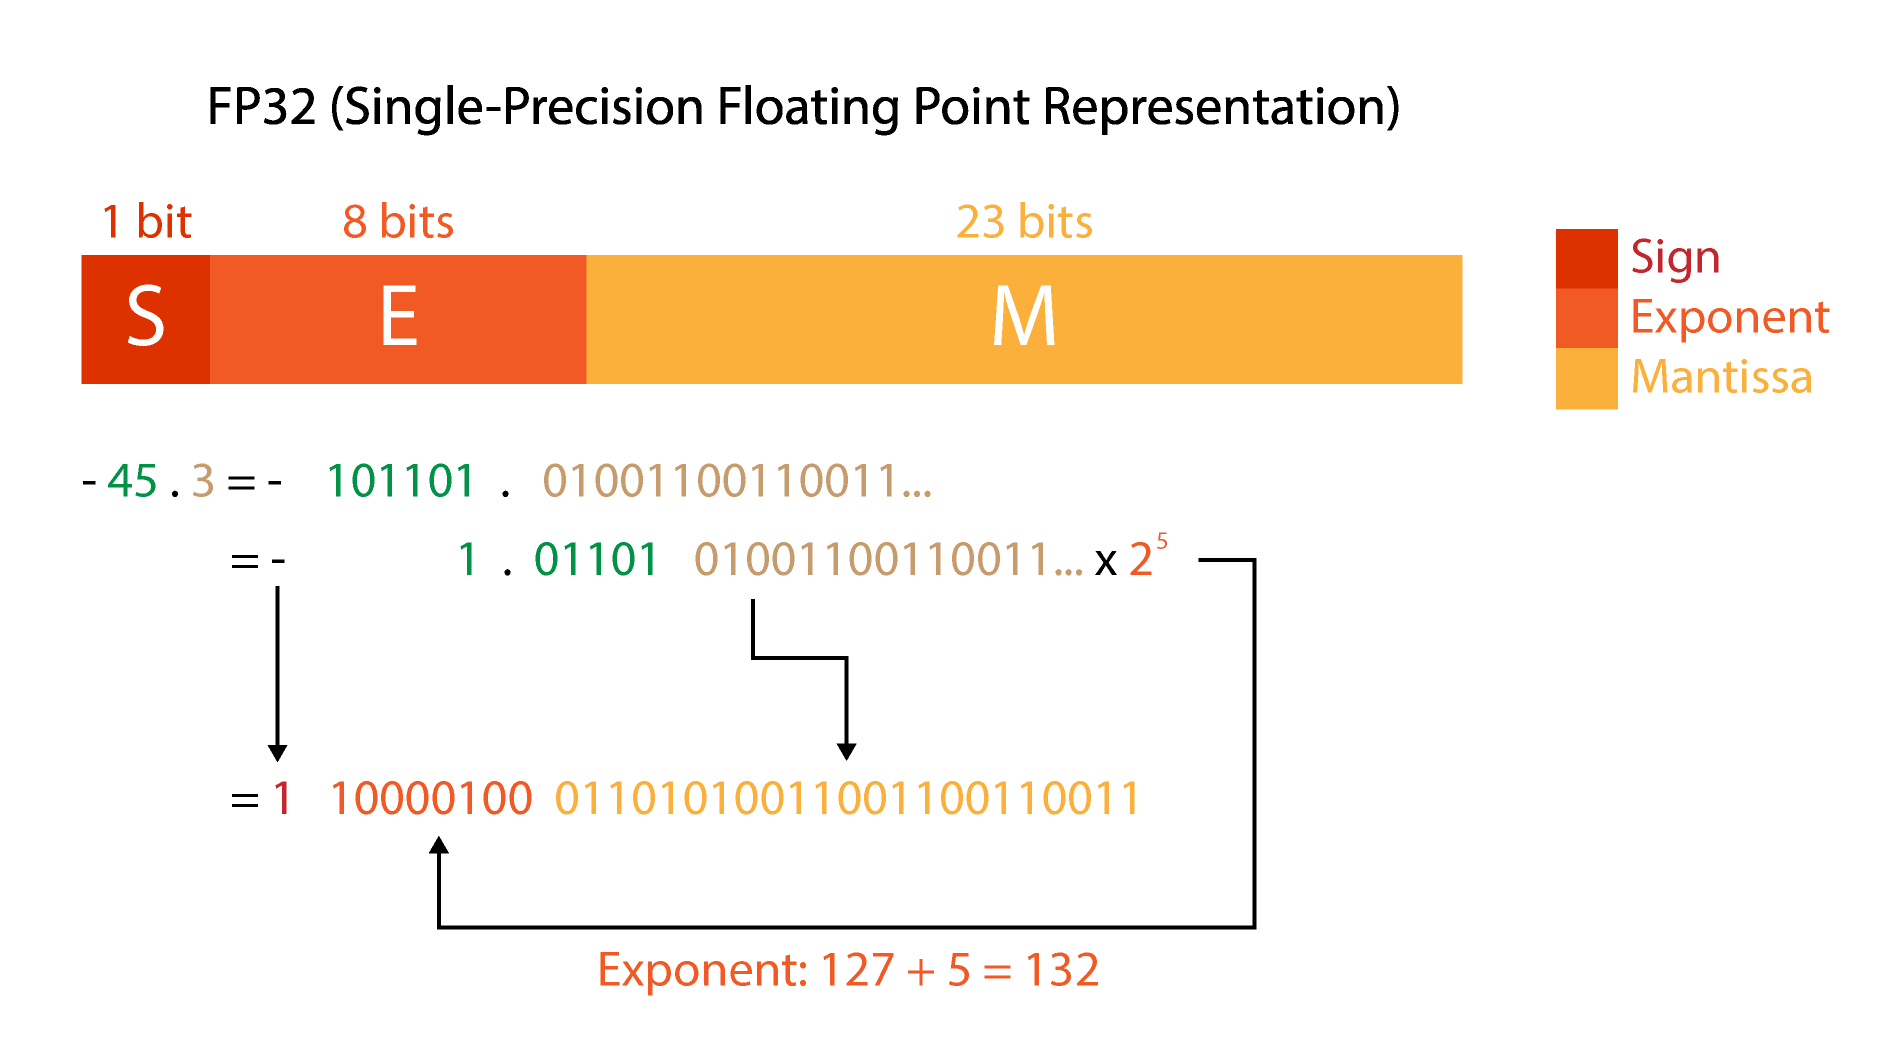
\includegraphics[width=.8\textwidth]{Figures/FP32.png}
	\caption[Single-precision float representation]{Example of the representation of a float in single-precision}
	\label{fig:FP32}
\end{figure}

Referring to double precision floating-point representation means looking at 64-bit long memory representation, mapped as follows and as shown in \emph{Figure} \ref{fig:FP64}:
\begin{itemize}
  \item Sign bit: 1 bit
  \item Exponent: 11 bits
  \item Mantissa: 52 bits
  \item Exponent Bias: 127
\end{itemize}

% FP64 EXAMPLE
\begin{figure}[htbp]
	\centering
		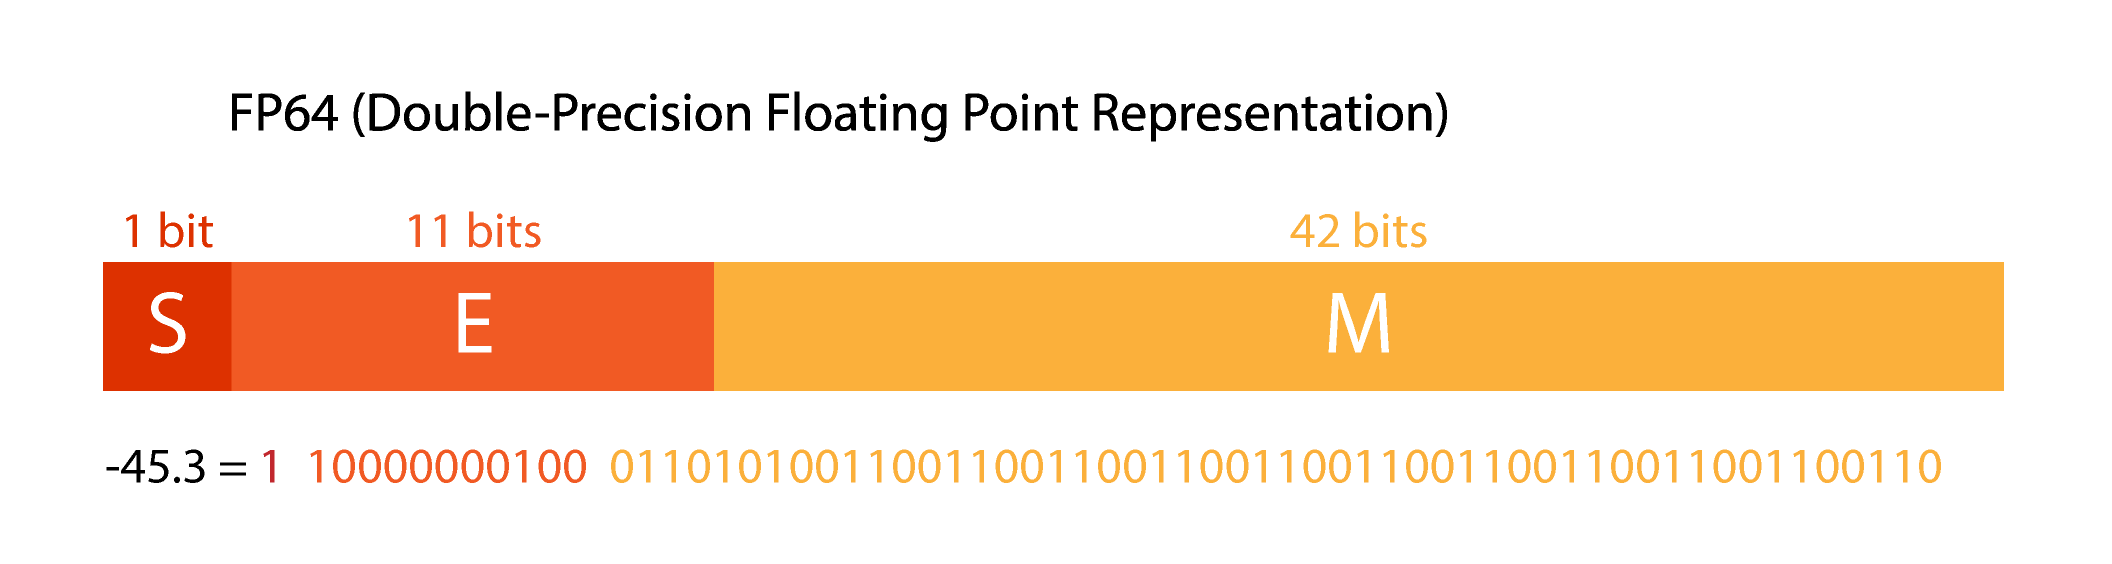
\includegraphics[width=.8\textwidth]{Figures/FP64.png}
	\caption[Double-precision float representation]{Example of the representation of a float in double-precision}
	\label{fig:FP64}
\end{figure}

Along these representations, IEEE-754 introduces representations of special numbers. Positive and negative infinities are encoded with all 1s exponents and a fraction equal to zero. Zero is encoded with an all-0s exponent and fraction. Moreover, it adds methods to round floating-point numbers to positive or negative infinity, zero or to the nearest value.

%-----------------------------------
%	SUBSUBSECTION 3 - Fixed-Point Representation
%-----------------------------------
\subsubsection{Fixed-Point Representation}

Another way to look at the decimals is to fix the radix point to be at a certain place and keep it throughout all the computations and representations using this arithmetic. A fixed-point representation consists of three components:
\begin{enumerate}
  \item A sign indicator
  \item An integer corresponding to the total number of bits
  \item Another integer corresponding to the size of the fractional part
\end{enumerate}

Representing a number with this representation can be done by simply concatenating the base 2 representation of each side of the radix point. This means the integer part will be represented with positive powers of two ($2^0$,$2^1$,$2^2$,...) while the fractional part is represented with negative powers of two ($2^{-1}$, $2^{-2}$,...).

% FIXED POINT EXAMPLE
\begin{figure}[htbp]
	\centering
		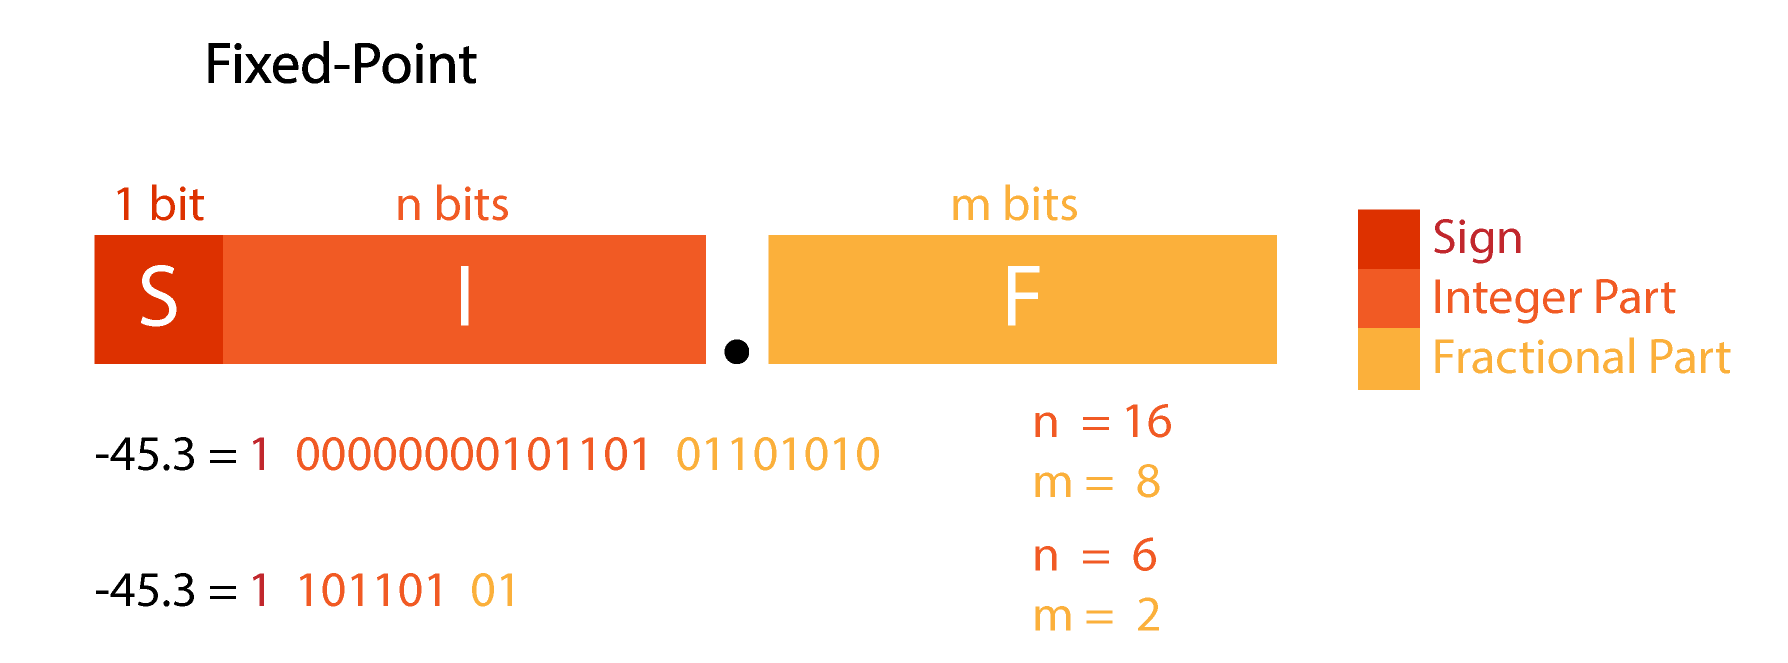
\includegraphics[width=.8\textwidth]{Figures/FixedPoint.png}
	\caption[Fixed-Point Representation]{Example of a float in fixed-point representation}
	\label{fig:FixedPoint}
\end{figure}

As shown in \emph{Figure} \ref{fig:FixedPoint}, several representations can depict the same decimal number. Finding the correct amount of bits to allocate to each side of the radix point is what will qualify the representation. Allocating fewer bits than needed may lead to overflow while allocating too much may increase quantisation errors.
Along with this new representation comes a whole new arithmetic. While this format can help tailor your needs in terms of variable types, it comes with an additional cost. The operations performed in this arithmetic are non-trivial as addition and multiplication are not associative and distributive anymore. This means the order of the operations will have an impact on the final result. Moreover, the round-off error underlying this representation is often non-trivial to grasp. However, those operations are low demanding in terms of computing power.

% PRESENT A WAY TO COMBINE DIFFERENT PRECISIONS

%-----------------------------------
%	SUBSECTION 2 - Performance Benchmarks
%-----------------------------------
\subsection{Metrics \& Performance benchmarks}

Floating-point representation (in either single or double precision) allows extreme precision at the cost of performance trade-offs (space or memory). On the other hand, fixed-point representation, even if it comes with a more complex arithmetic and insidious round-off errors, allows to tailor the type to your needs. Storing the values of the size and mass of planets in floating-point precision, would end up not using the majority of the range of values you selected while one could tailor a correct type in fixed-point representation.

The benchmarks in this field use several metrics in order to quantify and qualify the representations and their implementations.
\begin{itemize}
	\item \textbf{Size}: The size of a number in a given representation.
	\item \textbf{Energy cost}: The cost of operations in a given representation. \emph{The lower the better}.
	\item \textbf{Frequency}: The clock rate of a piece of hardware, or the quickness of pulses generation. \emph{The lower the better}.
	\item \textbf{Latency}: The access time of a piece of hardware to memory or external devices. \emph{The lower the better}.
	\item \textbf{Accuracy}: The precision enabled by a given representation. \emph{The higher the better}.
	\item \textbf{Memory Usage}: The memory needed to store both numbers and results of operations between them. \emph{The lower the better}.
	\item \textbf{Performance}: The overall time needed to complete a sequence of operations.
\end{itemize}

The operations performed in floating-point are expensive in terms of bandwidth, memory and energy consumption, which ultimately translate in to additional cost to perform an action. Horowitz's talk at ISSCC 2014 \cite{Horowitz2014} entitled \guille{Computing's Energy Problem (and what we can do about it)} provides an insight of the problems and challenges technology scaling has encountered in its development. Moore's law is getting outdated and a solution to the issue of permanently growing energy needs resides in \guille{the design of applications and hardware that are better matched to task and each other}. The numbers presented by M.Horrowitz have been reused by Professor William Dally (Standford University, NVidia Corporation) in his lecture on \guille{High-Performance Hardware for Machine Learning} \cite{Nips2015}. The \emph{Figure} \ref{fig:OpCosts} is extracted from this lecture and presents the energy and area costs different floating-point operations demand. Increasing precision on the used numbers increases the relative energy cost at the same time. An 8-bit addition costs 0.03 pJ whereas the same addition in 32-bit floating-point costs 0.9 pJ or 30 times more.

% COSTS OF OPERATIONS 2015-NIPS
\begin{figure}[htbp]
	\centering
		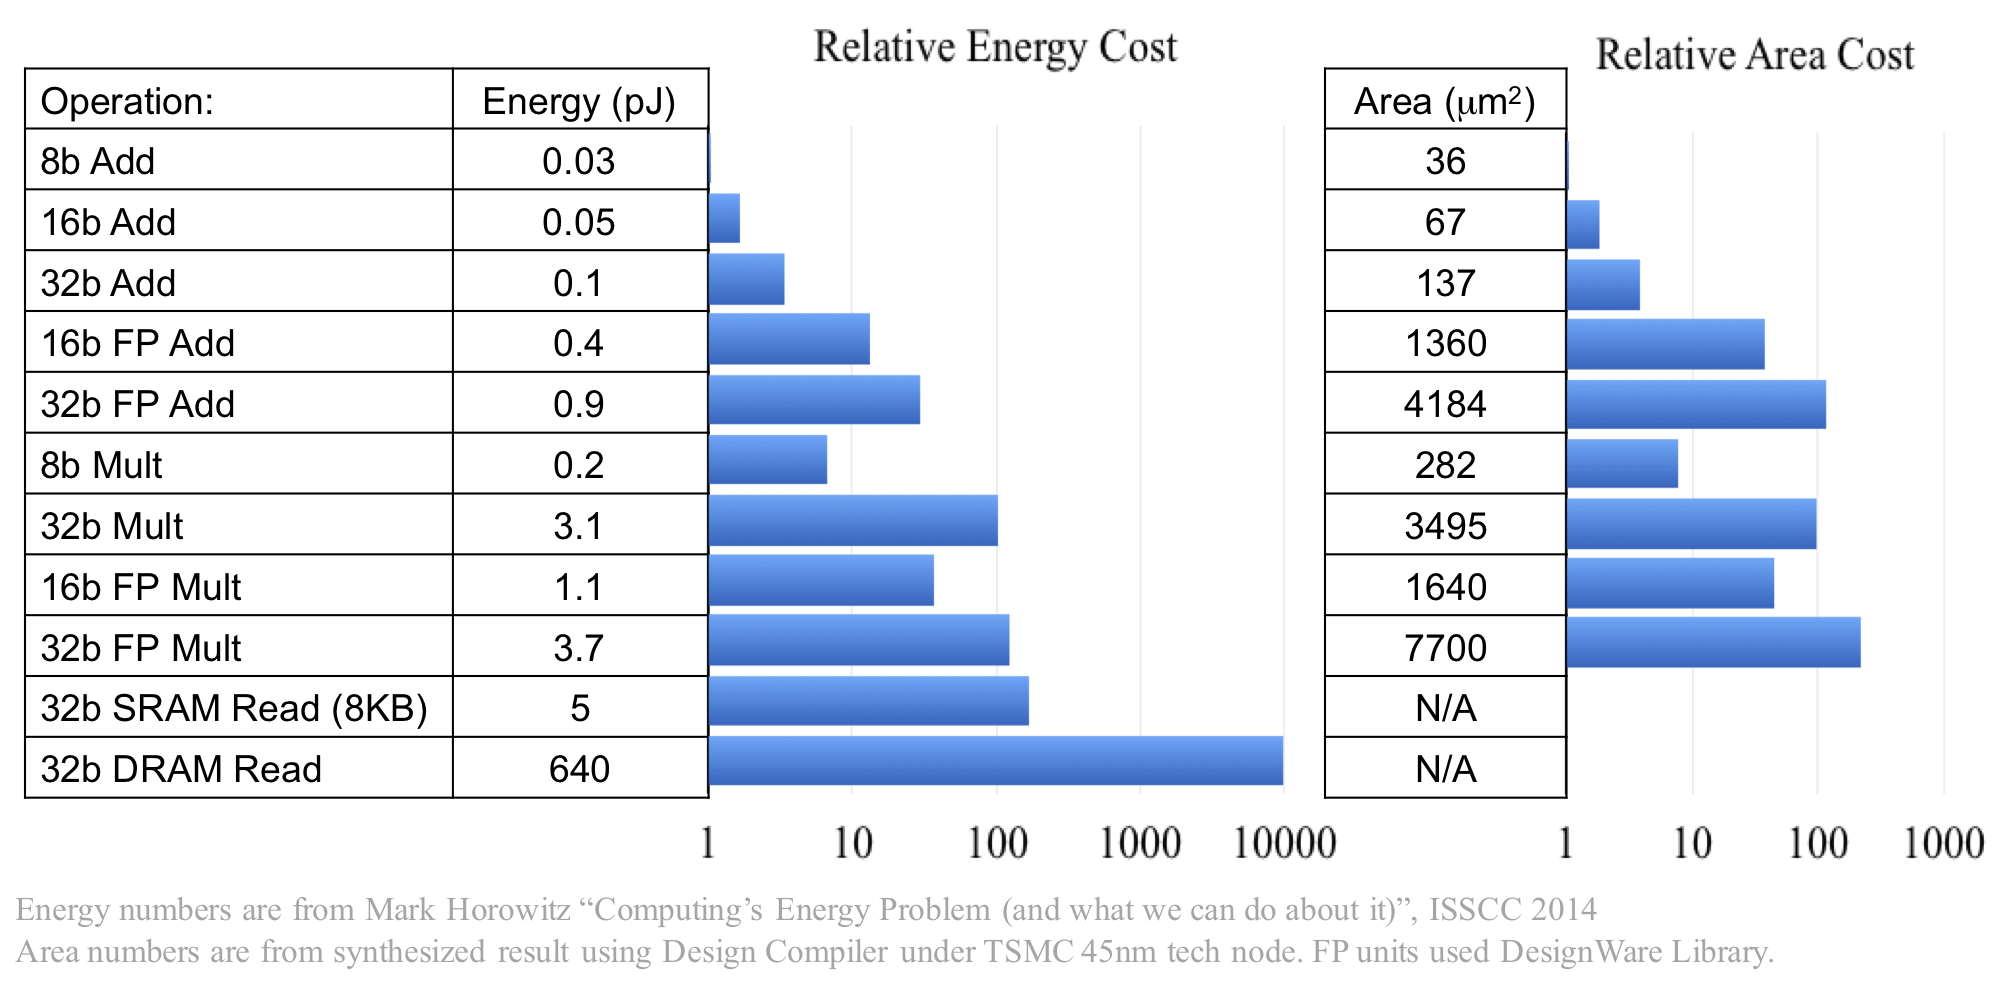
\includegraphics[width=\textwidth]{Figures/OpCosts.png}
	\caption[Operation costs]{Cost of operations in certain representations \cite{Nips2015,Horowitz2014}}
	\label{fig:OpCosts}
\end{figure}

The benefit of using a more optimised representation other the floating-point representation has been investigated as soon as in 2000 in \cite{Tong2000}. The authors present a way to reduce the energy consumption by minimising the bitwidth representation of the floating-point data. The data used to tailor the type representation is human-sensory data such as speech or video imagery. This kind of data is obtained at low precision (4 to 10 bits) but mapped into a full single-precision floating-point type. Using such optimisations, the authors manage to obtain a reduction of 66\% in multiplier energy per operation without sacrificing any accuracy.

Modifications of the representations can be embedded in the architecture. Xilinx, a manufacturer of state-of-the-art architecture, produced a white paper written by Finnerty et al. \cite{Xilinx2017} showing that their tools are able to handle fixed-point types and arithmetic and that the benefits are important:
\begin{itemize}
  \item Reduced power consumption
  \item Reduced use of resources (look-up tables, memory)
  \item Latency improvements
  \item Comparable performance and accuracy
\end{itemize}
The authors show the example of an FIR filter implementation in fixed-point representation from floating-point. The frequency is shown to be 16\% faster and the latency 7.5 times lower.

In conclusion, customising type in an environment where costs are translated in terms of energy consumption, memory or bandwidth usage, will always come out as an improvement. This redirects the issue to a need to guarantee little to no loss in accuracy.

%----------------------------------------------------------------------------------------
%	SECTION 2 - Background - Machine Learning
%----------------------------------------------------------------------------------------

\section{Background: On machine learning}


%----------------------------------------------------------------------------------------
%	SECTION 3 - Mixed Precision
%----------------------------------------------------------------------------------------

\section{Mixed Precision}

The previous section explained in details the different existing number representations. With a particular emphasis on the representation of floating-point number, it has shown which the underlying issues of such representations are. The question now is how can we use to our advantage the different types along with their strengths and weaknesses?

%-----------------------------------
%	SUBSECTION 1 - Motivations
%-----------------------------------
\subsection{Motivations}

The term \guille{mixed precision} comes from the idea of using different precisions (type representations) to increase the performance of a computation that would otherwise only use the highest available (or user-defined) precision. The previous section showed us that each number representation has its pros and cons. Using lower precision types and representations will allow the total computation to decrease the usage of several hardware resources (memory, bandwidth, energy consumption) \cite{Horowitz2014,Nips2015}.

However, if lower-precision is acceptable, using mixed-precision can increase the capacity of smaller systems and subsystems as it will increase the overall performance and resources usage. This goal is targeted when you are aiming for the most performant processor, being given a size and type of usage. Moreover, this can be used when you know exactly the tasks your system will perform as well as their needed size. Yates \cite{Yates2007} presents several rules allowing  to determine the required size of any operation performed in fixed-point arithmetic. This arithmetic allows to tailor the type size to one's needs. Reconfigurable hardware can take advantage of this as well by using the exact required size for an operation. Such architecture will be looked upon in the next sections.

Scientific computations often require the highest available precision and the reduced precision induced by the lower-precision components is unacceptable. In order to still take advantage of the several gains lower-precision provides, a compromise has to be found about how and when to use lower-precision. Ideas on the usage have been looked upon since the 1950's and the first methods to correctly implement them in the early 1960's.

In any case, the developer has to know and keep in mind:
\begin{itemize}
  \item Required end precision
  \item Acceptable error rate
  \item Actual operations performed by the system
\end{itemize}

Mixed precision methods consist of doing a large part of the computation in low-precision components and only a small part in high-precision. As presented in the survey paper \cite{Goddeke2007} using different formats in the same algorithm can have several beneficial properties such as:
\begin{itemize}
  \item Accuracy: Same accuracy when up to 99\% of the operations is performed in the low format
  \item Computation: Low precision operations require less transistors and can translate in more paralellism
  \item Memory: Reduction in size in memory influences the efficiency and bandwidth requirements positively
\end{itemize}

%-----------------------------------
%	SUBSECTION 2 - Methods and Implementations
%-----------------------------------
\subsection{Methods and Implementations}
Several methods to actually implement a mixed precision algorithm have been developed starting 60 years ago. If the methods are different in practice, the theory behind them is the same as they aim to delegate most of the work to low-precision components while only using high-precision to recover the desired accuracy for the computation.
%-----------------------------------
%	SUBSUBSECTION 1 - Iterative Refinement
%-----------------------------------
\subsubsection{Iterative Refinement}

Since the early 1960's, literature has studied the effects and ways to implement mixed precision. The first reported works to implement such methods are James H. Wilkinson \cite{Wilkinson1994} and Cleve Moler \cite{Moler1967}. The method presented by both is named \guille{iterative refinement} and uses a combination of accumulative inner products along with a linear solver. This solution is directed towards the resolution of a system in the form of $Ax=b$ for a quadratic $N*N$ matrix $A$. The main idea is to use a residual between the wanted result and the result obtained by the last iteration. This residual is computed using high precision and accumulated using high-precision as well while the resolution of the equation is done in low-precision.

% Iterative Refinement Example
\begin{figure}[htbp]
	\centering
\begin{tabular}{ll}
	$x^{(0)}=0$ &\\
	$d^{(s)}=b-Ax^{(s)}$ & Compute residual in \emph{high} precision\\
	$Ac^{(s)}=d^{(s)}$ & Solve equation system in \emph{low} precision\\
	$x^{(s+1)}=x^{(s)}+c^{(s)}$ & Accumulate solution in \emph{high} precision\\
\end{tabular}
	\caption[Iterative Refinement]{Iterative Refinement Method \cite{Goddeke2007}}
	\label{fig:IterativeRef}
\end{figure}

This method has later been reused and extended. Baboulin et al. \cite{Baboulin2009} combine single- and double-precision floating-point numbers to enhance the performance of \guille{dense and sparse linear algebra algorithms}. Strzodka et al. \cite{Strzodka2006} present an enhanced algorithm to resolve a partial differential equation (Poisson problem) to present the effects of a mixed-precision approach. Sun et al. \cite{Sun2008} reproduce a linear solver in mixed-precision but adds an error analysis. The last two articles implement the result of their research on a reprogrammable architecture. Several applications profit directly from these papers and their implementations of mixed-precision algorithms as seen in later sections.

\subsubsection{Analysis and Rewriting}

When creating a new application or system, any developer tends to use the highest available (or one of the highest) to represent the numbers he will need. However, the space and operations performed on higher-precision types are, as shown earlier, not the most performant. A simple, yet effective way to choose the correct type is to analyse the code and rewrite types that can be represented by lower precision ones. This idea has been implemented in the code analysis tool Precimonious \cite{Rubio2013} for floating-point representations. This analysis tool can go over the code and determines parts of it where lower precision can apply.

The mixed-precision approach can apply from a different perspective when using a fixed-precision representation. Darulova et al. \cite{Darulova2013} show that several polynomial expressions over the reals are cast over fixed-point arithmetic without being optimised, leading approximations of the real values. The tool they present allows to determine the best fixed-point implementation of a real number thanks to genetic programming. Then, as the order of operations is impactful when dealing with fixed-point arithmetic (distributivity and associativity are not respected), the tool reorder the operations to optimise the error and accuracy.

Those two tools have been brought together in \cite{Darulova2018} under the \guille{first fully automated and sound technique and tool for optimising the performance of floating-point and fixed-point kernels}. This tool combines rewriting and mixed-precision tuning where rewriting goes over several evaluation orders and picks the one that minimises the round-off error without runtime costs. In the meantime, mixed-precision tuning assigns the correct finite-precision variables and operations. The overall tool provides finer-grain control over the program and better performance than each of the method taken alone.
% TUNING EXAMPLE
\begin{figure}[htbp]
\centering
\begin{minipage}{.48\textwidth}
\begin{lstlisting}[style=CInputStyle]
long double fun( long double x ) {
  int k, n = 5;
  long double t1;
  long double d1 = 1.0L;
  t1 = x;
  for( k = 1; k <= n; k++ ) {
    d1 = 2.0 * d1;
    t1 = t1 + sin (d1 * x) / d1;
  }
  return t1;
}
int main( int argc, char **argv) {
  int i, n = 1000000;
  long double h, t1, t2, dppi;
  long double s1;
  t1 = -1.0;
  dppi = acos(t1);
  s1 = 0.0;
  t1 = 0.0;
  h = dppi / n;
  for( i = 1; i <= n; i++ ) {
    t2 = fun (i * h);
    s1 = s1 + sqrt (h*h + (t2 - t1)*(t2 - t1));
    t1 = t2;
  }
  // final answer is stored in variable s1
  return 0;
}
\end{lstlisting}
\end{minipage}
\hfill
\begin{minipage}{.48\textwidth}
\begin{lstlisting}[style=CInputStyle]
double fun( double x ) {
  int k, n = 5;
  double t1;
  float d1 = 1.0f;
  t1 = x;
  for( k = 1; k <= n; k++ ) {
    d1 = 2.0 * d1;
    t1 = t1 + sin (d1 * x) / d1;
  }
return t1;
}
int main( int argc, char **argv) {
  int i, n = 1000000;
  double h, t1, t2, dppi;
  long double s1;
  t1 = -1.0;
  dppi = acos(t1);
   s1 = 0.0;
  t1 = 0.0;
  h = dppi / n;
  for( i = 1; i <= n; i++ ) {
    t2 = fun (i * h);
    s1 = s1 + sqrt (h*h + (t2 - t1)*(t2 - t1));
    t1 = t2;
  }
  // final answer is stored in variable s1
  return 0;
}
\end{lstlisting}
\end{minipage}
\caption[Tuning]{Tuning Example \cite{Rubio2013}}
	\label{fig:Tuning}
\end{figure}

%----------------------------------------------------------------------------------------
%	SECTION 3 - Application
%----------------------------------------------------------------------------------------

\section{Applications}

Mixed-precision mindset and algorithms are used in several applications from overall performance boosting due to precise tuning to new methods to handle tomorrow's problematics such as Big Data or Deep Learning. The question to ask when developing a new application that can benefit from mixed-precision is: how to put it in action inside an application? Code analysis and rewriting? Finer-grain tuning or more complex algorithms such as the earlier iterative refinement?

%-----------------------------------
%	SUBSECTION 1 - Linear Algebra
%-----------------------------------

\subsection{Mathematic computations}

Linear Algebra directly gains from iterative refinement techniques and can be applied to several wider projects. Some well-known linear problems and operations are the bottleneck of their container projects and finding an optimisation leading to a better performance in their resolution would mean a direct improvement to the overall performance. Baboulin et al. \cite{Baboulin2009} and Sun et al. \cite{Sun2008} present a mixed-precision method aiming at the LU factorisation.
\begin{align}
  PA=LU \textrm{ where } & \textrm{A is the matrix to factorise} \\
        & \textrm{P is a permutation matrix} \\
        & \textrm{U an upper triangular matrix} \\
        & \textrm{L is a lower triangular matrix}
\end{align}
This factorisation is required in many different algorithms using linear algebra as obtaining triangular matrices simplifies later computation. While both authors focus on the same subject, \cite{Sun2008} presents a reconfigurable architecture design and implementation. Later on, Haidar et al., a group of researchers and NVidia CUDA library engineers, showed a 4 times performance improvement in \cite{Haidar2018} and \emph{Figure} \ref{fig:HaidarPerf}.

% PERFORMANCE IMPROVEMENT HAIDAR 2018
\begin{figure}[htbp]
	\centering
		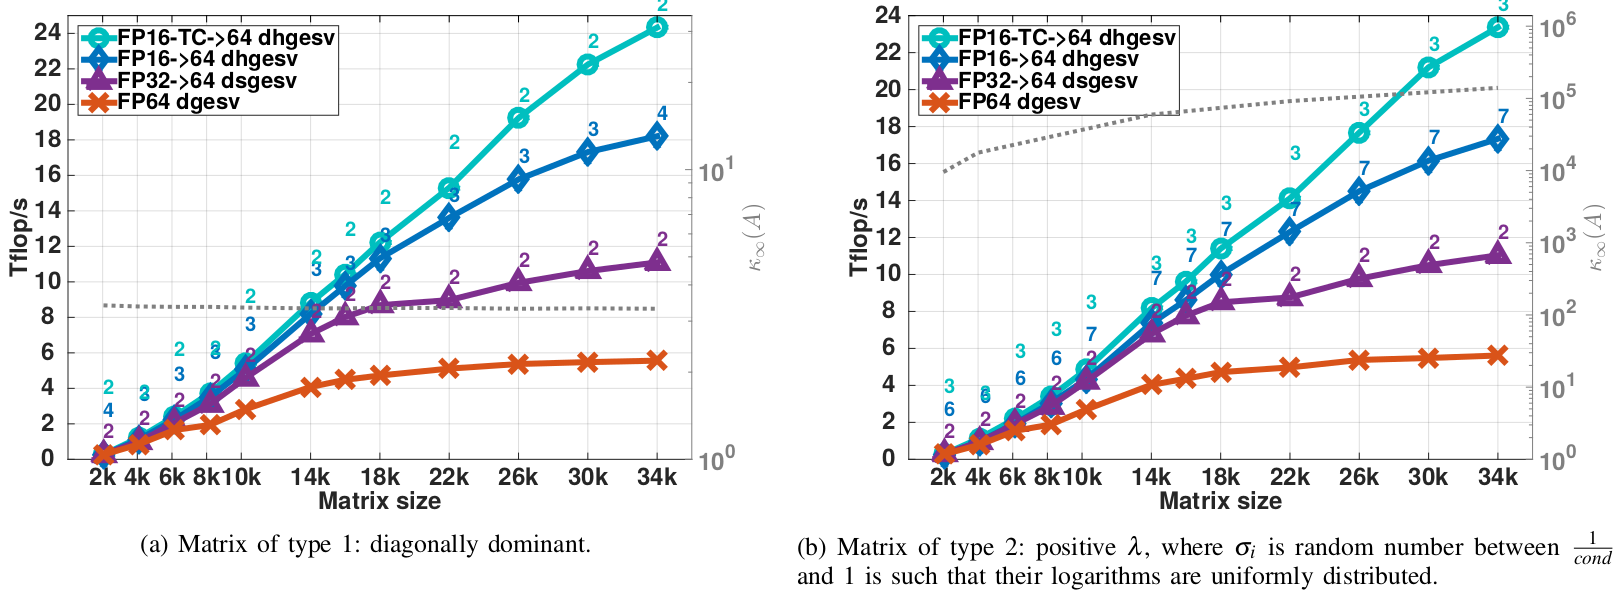
\includegraphics[width=\textwidth]{Figures/HaidarPerf.png}
	\caption[Performance Improvement]{Performance Improvement of the LU factorisation \cite{Haidar2018}}
	\label{fig:HaidarPerf}
\end{figure}

Strzodka et al. \cite{Strzodka2006} present a solution to the partial differentiate equation Poisson problem defined on a reconfigurable architecture. The resolution of such a problem is done using methods called multi-grid solvers or the simpler conjugate gradient solver. The mixed-precision is integrated in the solution process by splitting it into a \guille{computationally demanding low precision inner iteration loop and a computationally simple high precision outer correction loop}. The authors present different pipelined versions of the conjugate gradient solver that focus on parallelisation.

Another mathematic computation extensively used in the world of science, engineering and finance are Monte Carlo simulations that are used to simulate random processes and estimate the distribution of the results. Chow et al. \cite{Chow2012} present a mixed-precision version of the sampling function used in the Monte-Carlo simulation. Along with the solution, the authors provide a description of the hardware implementation made possible on reconfigurable architecture.

%-----------------------------------
%	SUBSECTION 2 - Simulations (Physics)
%-----------------------------------

\subsection{Physics simulations}

A direct application of the above computations is the improvement of physics simulations. Such simulations are usually done using GPUs  and can take place in several fields requiring computationally intensive operations. Such fields are molecular chemistry, nuclear physics and finite element simulations for example.

Goddeke et al. \cite{Goddeke2007} present a survey paper to quantify the performance and accuracy of mixed-precision solvers in finite element simulations. This survey paper takes in consideration different mixed precision algorithms and their associated implementations. Moreover, it compares the performance of different hardware architecture, CPUs, GPUs and FPGAs. The article confirms that low-precision operations are more performant but need the developer to have knowledge of the error propagation. Finite element simulation is a method used to split a bigger object in smaller parts and define the interactions between them. It can be visualised as shown in \emph{Figure} \ref{fig:FESim}.

% FINITE ELEMENT SIMULATION
\begin{figure}[htbp]
	\centering
		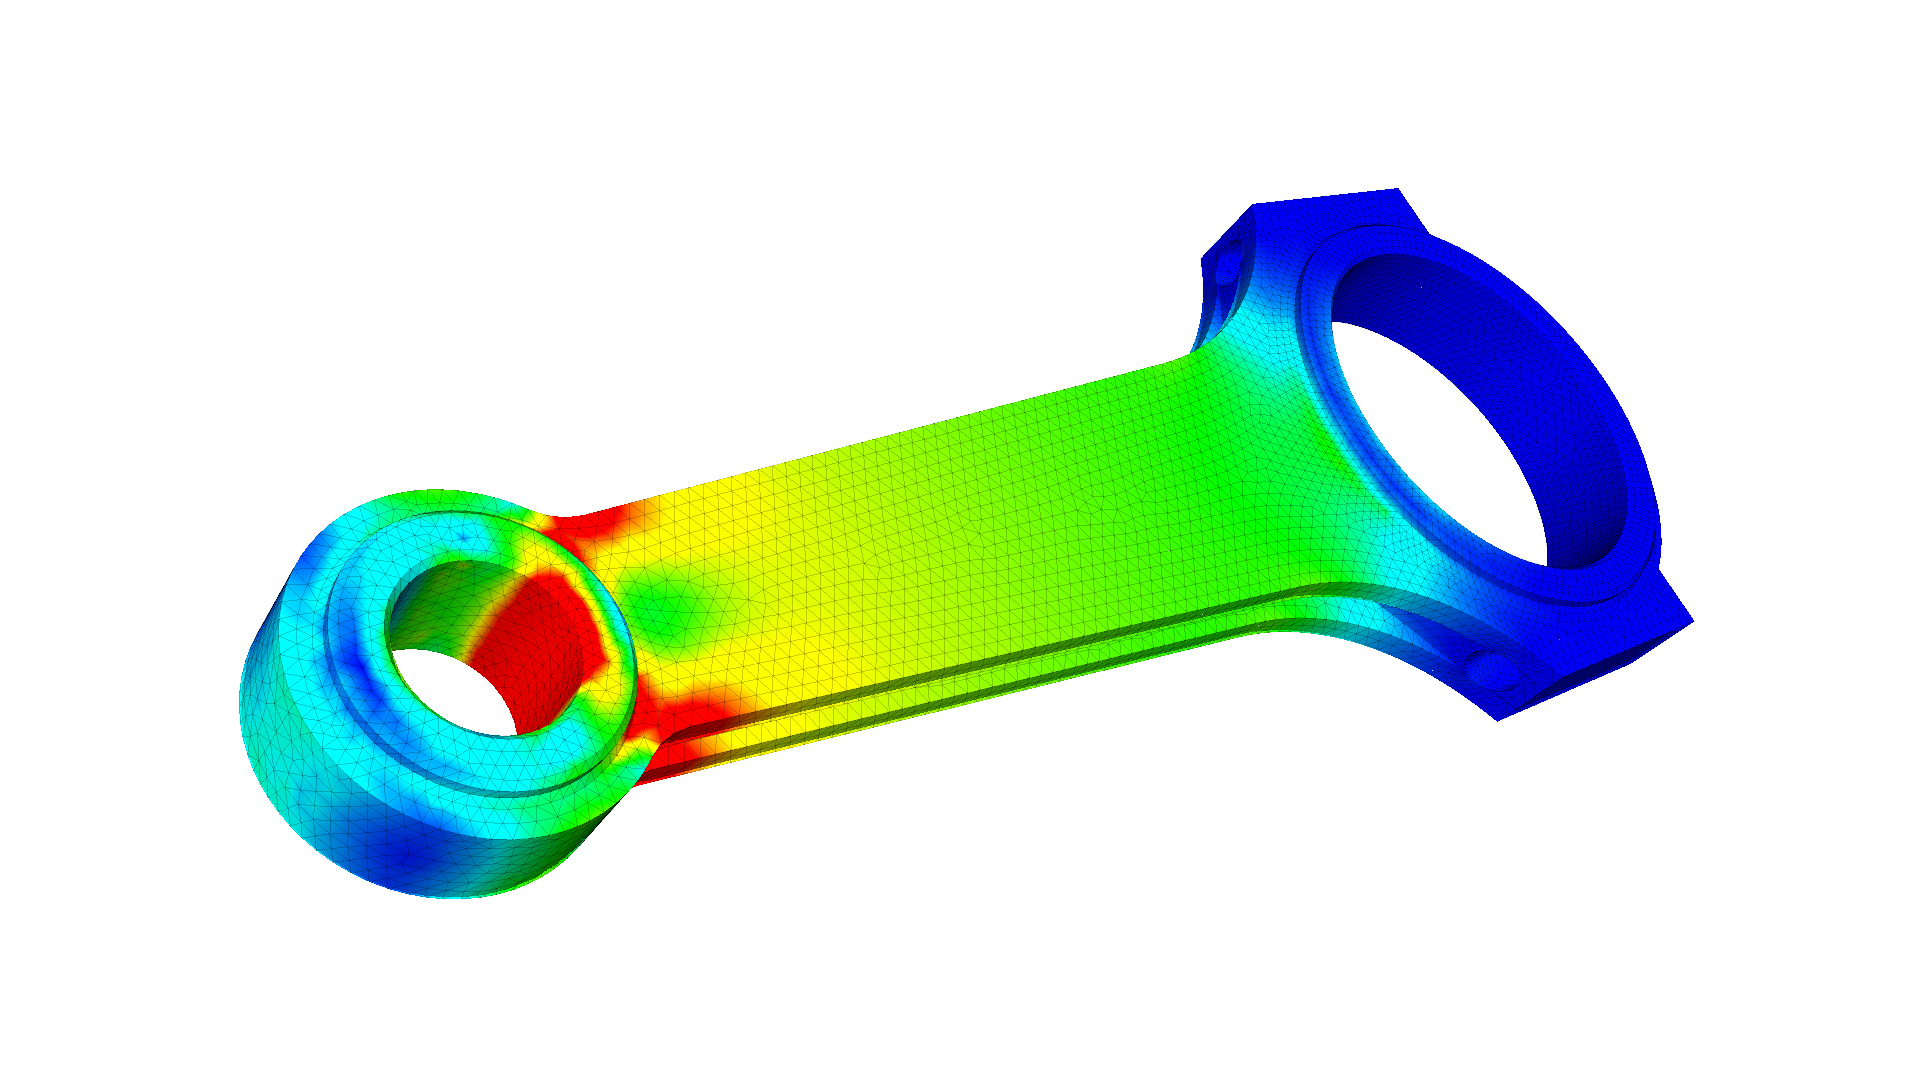
\includegraphics[width=.5\textwidth]{Figures/FESim.png}
	\caption[Finite Element Simulation]{Finite Element Analysis of a piston rod \cite{Simscale}}
	\label{fig:FESim}
\end{figure}

In the same finite element simulation field, Ichimura et al. \cite{Ichimura2018} present a mix between mixed-precision and artificial intelligence through an earthquake simulator. They managed to get finalist in the Supercomputing 2018 conference (SC'18). The AI is used to improve the convergence of the solver and the use of reduced precision improves the performance by 25.3 over a standard solver and by 3.9 times over a previous state-of-the-art solver (SC'14). This improvement was made with no loss in accuracy.

% EARTHQUAKE SIMULATION
% \begin{figure}[htbp]
% 	\centering
% 		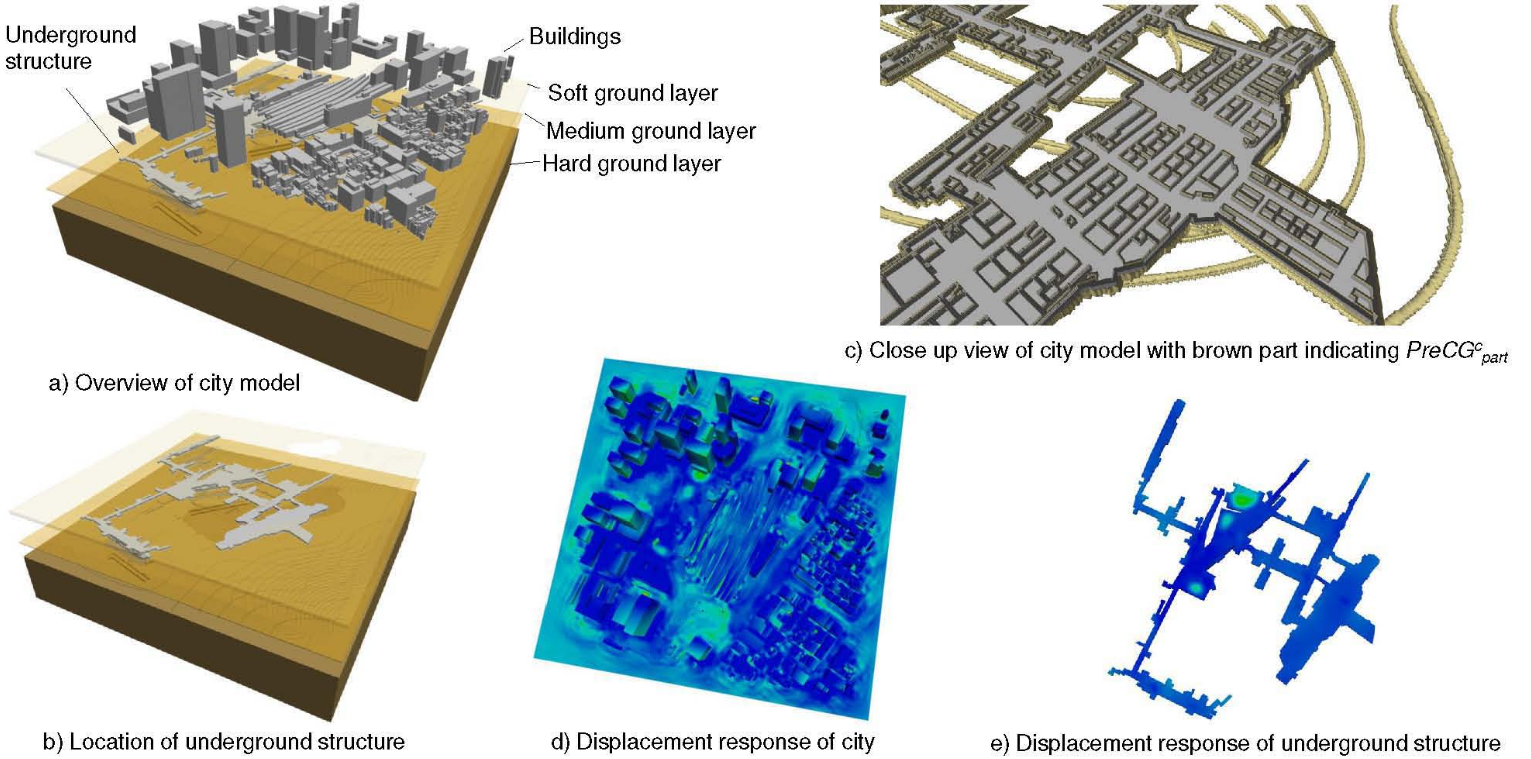
\includegraphics[width=\textwidth]{Figures/EarthquakeSim.png}
% 	\caption[Earthquake Simulation]{Earthquake simulation created with AI and mixed-precision \cite{Ichimura2018}}
% 	\label{fig:EarthquakeSim}
% \end{figure}

Clark et al. \cite{Clark2010} use mixed-precision to solve lattice quantum chromodynamics systems of equations in simulations. These systems corresponds to \guille{the lattice discretised theory of the strong force, that which binds together quarks in the nucleon}. The propagation of those quarks uses a Dirac operator's inverse, a large sparse matrix that needs to be used in several system of operations later on. The Wilson-Dirac matrix is the target of the optimisation and this optimisation is made possible by implementing a method of mixed-precision using \emph{reliable updates} within a linear solver. Those \emph{reliable updates} periodically replace the iterated residual with the true residual calculated at high precision and allows better performance than classic defect-correction approach.

% QUARK SIMULATION
% \begin{figure}[htbp]
% 	\centering
% 		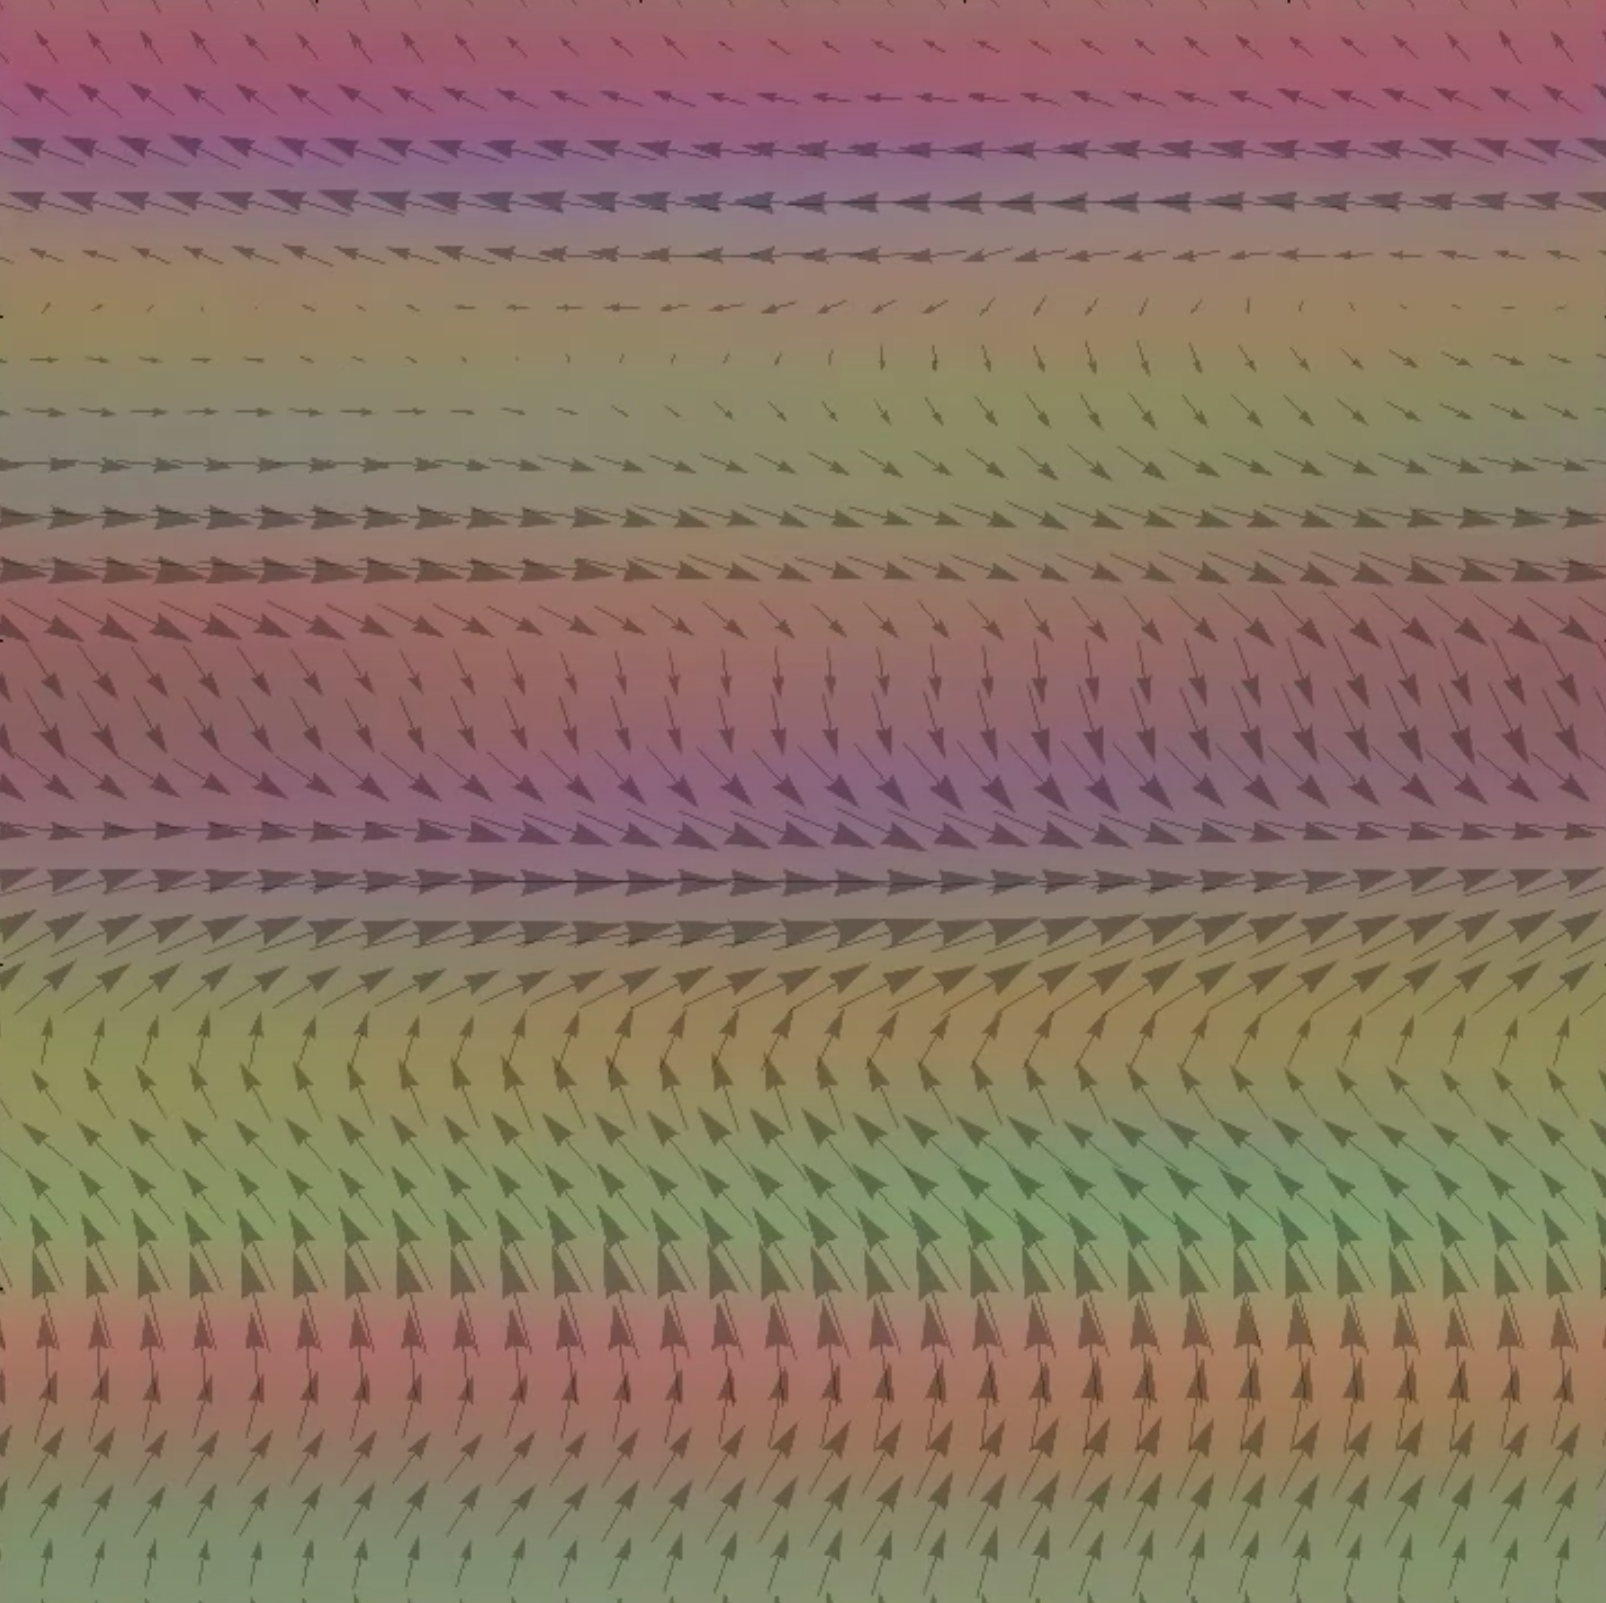
\includegraphics[width=.3\textwidth]{Figures/QuarkSim.png}
% 	\caption[Quark Simulation]{Simulation of Quark-Gluon Plasma Instabilities \cite{Ipp2011}}
% 	\label{fig:QuarkSim}
% \end{figure}

Molecular dynamics simulations are also using mixed-precision techniques as proposed by Le Grand et al. \cite{LeGrand2013}. The mixed-precision approach presented in the article uses fixed-point integer arithmetic to translate the force components. The article compares single precision fixed-point representation to the classic single/double precision. The conclusions show a gain in performance without sacrificing any accuracy.

% MOLECULAR DYNAMICS SIMULATION
\begin{figure}[htbp]
	\centering
		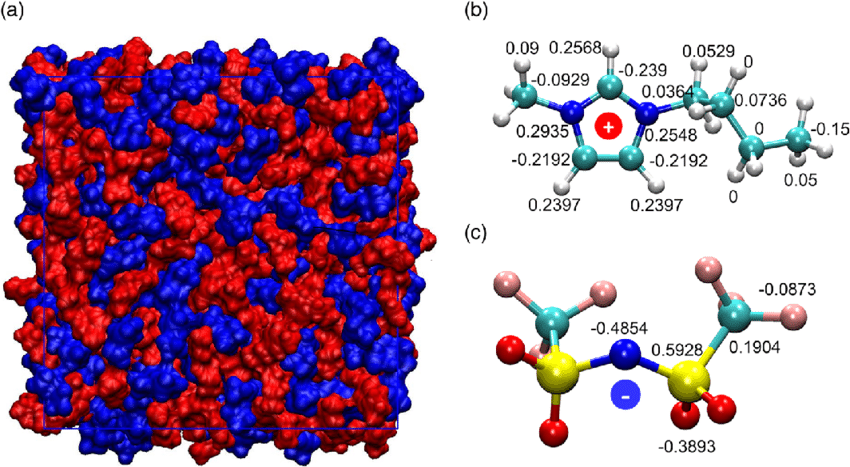
\includegraphics[width=.7\textwidth]{Figures/MolecularSim.png}
	\caption[Molecular Dynamics Simulation]{Molecular Dynamics Simulation \cite{Feng2019}}
	\label{fig:MolecularSim}
\end{figure}


%-----------------------------------
%	SUBSECTION 3 - Deep Learning
%-----------------------------------
\subsection{Deep Learning}

Machine learning can also benefit from mixed-precision since it is heavily relying on matrix operations. In the recent years, machine learning, and especially deep learning, are benefitting from the research in mixed-precision. As there is a lot of interest going in the performance of neural networks and their ability to train quicker and still be accurate, the focus of both fields appear to be extremely similar.

%-----------------------------------
%	SUBSUBSECTION 1 - Deep Learning
%-----------------------------------

\subsubsection{Neural Networks}

 Karpathy et al. \cite{Karpathy2015} present the different structures in their lecture materials. The apparition of neural networks in machine learning comes from the analogy with the human brain and the way neurons work and communicate between each other. The analogy can be seen on \emph{Figure} \ref{fig:Neuron}.

% NEURON PRESENTATION
\begin{figure}[htbp]
	\centering
		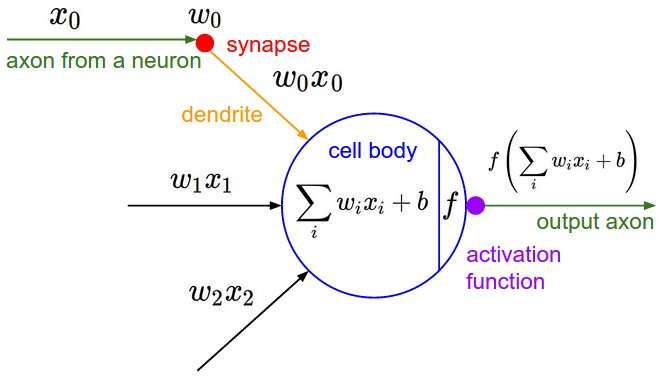
\includegraphics[width=8cm]{Figures/Neuron.png}
	\caption[Neuron Example]{Example of a neuron and its behavior in a neural network \cite{Karpathy2015}}
	\label{fig:Neuron}
\end{figure}

Each neuron receives several inputs from other previous neurons and performs an operation on all the received inputs to create the output that will go to its successors. A family of neurons that will obtain the outputs of the same neurons is called a \emph{layer}. A combination of \emph{layers} composes a \emph{neural network} as presented on \emph{Figure} \ref{fig:NN}.

% NEURAL NETWORK PRESENTATION
\begin{figure}[htbp]
	\centering
		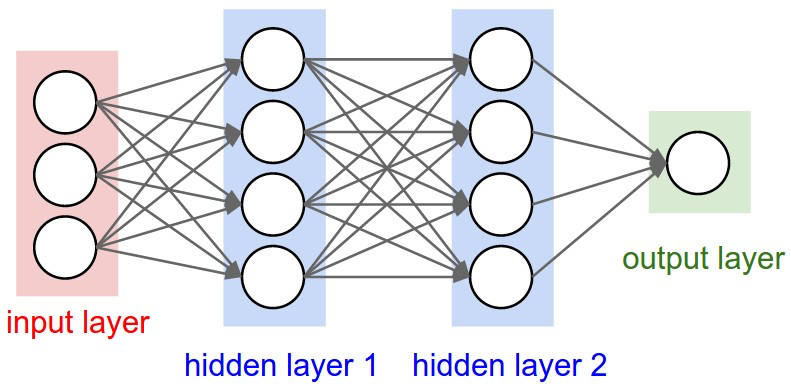
\includegraphics[width=8cm]{Figures/NN.png}
	\caption[Neural Network Example]{Example of a neural network architecture \cite{Karpathy2015}}
	\label{fig:NN}
\end{figure}

The neuron performs a simple dot product of all the inputs along with their weights, adds a bias to the sum and applies a given non-linear activation function. The weight will give importance to some of the inputs while hiding others. Throughout the training, some of the inputs will be shown to be more useful than others and their weight will depict this attribute. The activation function models the \guille{firing rate of the neuron which [...] represents the frequency of the spikes along the axoms}. Several choices of non-linear functions can be made for your neurons:
\begin{itemize}
  \item Sigmoid function: $\sigma(x) = \frac{1}{(1+e^{-x})}$
  \item Tanh: $tanh(x) = 2\sigma(2x) - 1$
  \item Rectified Linear Unit (ReLU): $ f(x) = max(0,x) $
\end{itemize}

Neural networks perform the simple operations of reducing the inputs, adding a bias and passing it through a non-linear function. However, it is possible to set up several layers where the first one is called the \emph{input layer}, the last one the \emph{output layer} and all the layers in-between the \emph{hidden layers}. These layers go one after each other as shown in \emph{Figure} \ref{fig:NN}. While having hidden neurons is useful to better comprehend the data fed to the network, having too much of them can lead to overfitting, including noise and outliers into the pattern recognition.

Neural networks perform well in machine learning, but the fields where the architecture is mostly used are image and speech recognition. An extension of neural networks is used when the data is known to be of a certain type. For example, if the data is known to be images, Convolutional Neural Networks (CNN) are the best choice as they are tailored with the goal of handling images. They are a special type of neural networks in the sense that they use 3D layers and transformations on images. CNNs can be used for image classification, object detection, image segmentation or speech recognition. We will focus on image recognition here as this field provides well-known metrics and network layouts due to the popularity of the ImageNet Project for example \cite{ImageNet2009}. This popularity has attracted literature focus and allows comparisons to be made.

% NEURAL NETWORK PRESENTATION
\begin{figure}[htbp]
	\centering
		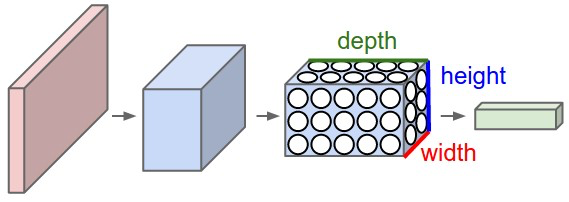
\includegraphics[width=8cm]{Figures/CNN.png}
	\caption[Convolutional Neural Network Example]{Example of a convolutional neural network architecture \cite{Karpathy2015}}
	\label{fig:CNN}
\end{figure}

Several layers are used and allow to perform different operations on images:
\begin{itemize}
  \item INPUT: Image input holding the resolution and RGB layers
  \item CONV: Connects small regions of the input image
  \item RELU: Apply an activation function (such as $max(0,x)$)
  \item POOL: Downsampling operation
  \item FC (fully-connected): Computation of the class scores
\end{itemize}

Layers input a set of data, known as a \emph{Feature Map} and output a new set of feature maps with higher-level semantics. Those layers then compose a CNN architecture and can be trained on a bank of images to adjust the different bias and weight for each layers. Finally, once the network is trained, it can deduce the class of a given image. Those two steps are called \emph{Training} and \emph{Inference}, the training will work on a set of annotated data samples to create a model \guille{which semantics extrapolate outside the training set, [with a] \emph{modelling power}} \cite{Abdelouahab2018}. Once this step is completed, the \emph{Inference} phase can start and the network will have to classify new data instances. This inference has to be run each time a new instance is provided to the system. Therefore, literature focus on accelerating this phase.

%-----------------------------------
%	SUBSUBSECTION 2 - Introducing Mixed Precision
%-----------------------------------

\subsubsection{Introducing Mixed Precision}

Training a neural network is the longest process, among mandatory ones, to make the most out of the architecture. However, mixed-precision mindset offers ways to accelerate the training of the network by decreasing the precision of some operations. The ImageNet Project \cite{ImageNet2009} is a large database designed to be used in visual object recognition softwares. The same project runs an annual contest, the ImageNet Large Scale Visual Recognition Challenge (ILSVRC). Every year, contesters try to get the best possible accuracy out of the network they propose. While accuracy is the main factor to determine the winner, deep learning real-world issues often have to take in account the network's training phase.

The benchmarks in this field use several metrics in order to quantify and qualify the networks and their implementations.
\begin{itemize}
	\item \textbf{Parameters' Size}: The size of parameters of the network: weights and activation functions.
	\item \textbf{Network Layout}: The configuration of the neural networks with the number, size and type of layers.
	\item \textbf{Accuracy}: The ratio of the number of correct precisions out of the total number of predictions. \emph{The higher the better}.
	\item \textbf{Training Time}: The cost of operations in a given representation. \emph{The lower the better}.
\end{itemize}

Many researchers have been looking into the issue with mixed-precision in mind. As shown by Bacchus et al. \cite{Bacchus2020}, there is a fundamental underlying trade-off between accuracy, network training time and hardware efficiency. Research looked upon ways to reduce the size taken by weights and the activation function and the impact of a reduction in the size of those:

Micikevicius et al. \cite{Micikevicius2017} store weights, activations and gradients in IEEE half-precision nearly halving the memory requirements and speeding up the arithmetic. The authors propose three techniques to maintain the accuracy of the model. They maintain a single-precision copy of weights to accumulate the gradients, propose a loss-scaling to preserve low-magnitude gradients and use half-precision arithmetic that writes to single-precision arithmetic before writing the half-precision values to memory.

Colangelo et al. \cite{Colangelo2018} present a CNN mapping to a reconfigurable architecture in order to use sub 8-bit activation and weights. In order to use binary- or ternary-weighted neural networks, they cap their sizes to respectively 1 and 2-bits. Using this type of limited numeric precision can only be fully optimised with FPGAs and the authors show that they manage to get an optimisation of \guille{the bandwidth, memory, power and computation savings}.

Jia et al. \cite{Jia2018} present a novel mixed-precision training method along with an optimised all-reduce algorithm. Any neural network will have to use a version of an all-reduce algorithm, consisting of the sum of all the previous elements broadcasted to all the next elements. Using an optimised version of the algorithm will increase the performance of each layer separately and the whole system in the end.

Zhao et al. \cite{Zhao2016} propose F-CNN, a framework to train CNNs on FPGAs. Their design makes available highly customisable modules that will be optimised to maximise performance under the constraints of bandwidth and hardware resources. The authors state that the introduction of mixed-precision will be the next step of optimisation of their design. Moreover, the use of they prove their design is more performant than CPUs and less expensive in terms of energy than GPUs.

Jahanshahi et al. \cite{Jahanshahi2019} propose a CNN accelerator tool. It generates the hardware description for a CNN to be programmed on a target FPGA. The software uses an API the developer can use to enter the available resources. The software will then generate the hardware description and run a simulation to adjust the precision and minimise the classification error. The whole system is shown to be more performant on a half-precision fixed-point representation rather than using single-precision floating-point data: 3\% accuracy loss in exchange for 15.75x speedup.

Kurth et al. \cite{Kurth2018} presents a direct application of mixed-precision training on GPUs to help climate analysis. The authors expand open-source tools such as Tensorflow and Horovod in order to present their work. They managed to optimise the network's training to increase the overall efficiency and performance. The predictions the network is able to make are shown to be of an unmet precision and will help characterise the impact of several physical events (flooding, monetary loss, etc.).

%----------------------------------------------------------------------------------------
%	SECTION 4 - Hardware Architecture
%----------------------------------------------------------------------------------------

\section{Hardware Architecture}

Moore's law \cite{Moore2006} predicted the evolution of hardware capacities in years to come when defined in 1965. It is an empirical relationship and in no means a physical or natural law but has shown to be exact for the thirty years following its creation. The Moore's law, when announced in 1965 said that \guille{the number of components per integrated circuit would double every year}. This law held for a decade and was then revised to \guille{doubling every two years} for the next decade. This law has been an industry guideline and helped produce long term business plans. However, the law is slowly coming to an end and has been shown to not fulfill the prophecy anymore due to physical limitations such as thermal restrictions. New architectures will have to take the lead as more computational power is still needed for the years to come. What are the new ways and architectures to increase performance even more?

%-----------------------------------
%	SUBSECTION 1 - GPU
%-----------------------------------

\subsection{GPU}

One solution to enable hardware acceleration is to parallelise computationally expensive tasks. GPUs (\emph{Graphics Processing Units}) are specialised electronic circuits that can handle computationally demanding tasks such as 3D rendering, video encoding and decoding or any action that can be massively parallelised (cryptocurrency digging, matrix computations or brute-force cracking). Few companies actually conceive and sell such systems. The most famous are NVidia, AMD and Intel and some smaller fabless - conceive the circuit but integrally subcontract the production -  companies such as Qualcomm or ARM. Other manufacturing companies such as ASUS or MSI will then integrate those circuits into products and calibrate them along with a cooling system that can make it enhance its base abilities.

Along with GPUs come their proper Software Development Kit (SDK) in order for developers to use their tools. NVidia invested heavily in CUDA (\emph{Compute Unified Device Architecture}) \cite{CUDA} and its aim is to reproduce a C syntax and environment for GPUs. AMD and Intel provide open-source SDK that tools then built upon.

GPUs allow computers to delegate expensive tasks (3D rendering for example) from the CPU to them. The GPUs can be either integrated or external. They require less knowledge than FPGAs but provide a more static architecture that will limit tuning opportunities. Mixed-precision mindset will not reach its full potential with this architecture but will still manage to increase the performance of different operations and tasks.

Previous cited works have used CPUs, in mathematical computations and physics simulations \cite{Goddeke2007, Baboulin2009, Clark2010, LeGrand2013, Haidar2018, Ichimura2018} or deep learning \cite{Goddeke2007, Baboulin2009, Micikevicius2017, Jia2018, Ichimura2018}.

%-----------------------------------
%	SUBSECTION 2 - FPGA
%-----------------------------------

\subsection{FPGA}

On the other hand, the 1990's have seen the birth of a new type of architecture: reconfigurable hardware. They allow to create application-specific hardware and are mixed-precision by default. Xilinx, one of the most famous FPGA manufacturer describes them as consisting of \guille{up to two million logic cells that can be configured to implement a variety of software algorithms} \cite{Xilinx2017}. Those logic cells can be dynamically reconfigured and this is the strength of this architecture.

FPGAs consist of several important elements:
\begin{itemize}
  \item Look-up table (LUT): component that performs logic operations.
  \item Flip-Flop (FF): register  for the results of the LUT.
  \item Wires: elements connectors.
  \item Input/Output (I/O) pads: physical ports to get data in and out of the FPGA.
\end{itemize}

Along with those base components come many high-end more interesting components that can help develop your hardware to be tightly linked to the application you have in mind. As stated by \cite{Goddeke2007}, FPGAs have native mixed-precision processors and \guille{there is no need to utilise the same number format throughout the algorithm, or even the same operation}. Moreover, the freedom in the number representation can lead to alternative feasible number representations, such as a logarithmic one.

One downside of FPGAs is the need for intrinsic knowledge of a Hardware Description Language (HDL) or one of their higher-level abstractions \cite{XuanSang2014}. While this step can be a downside, it also brings up a new layer of customisation, tuning and tests. The whole development cycle shown in \emph{Figure} \ref{fig:FPGACycle} can be controlled using a high-level development language such as Smalltalk in \cite{XuanSang2014}. Finer-grain tuning can be performed using the direct HDL language but the learning curve is steeper.

% FPGA Development Cycle
\begin{figure}[htbp]
	\centering
		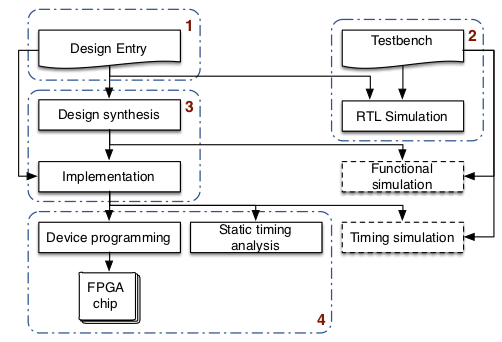
\includegraphics[width=\textwidth]{Figures/FPGACycle.png}
	\caption[FPGA Development Cycle]{FPGA Development Cycle \cite{XuanSang2014}}
	\label{fig:FPGACycle}
\end{figure}

%-----------------------------------
%	SECTION 5 - CNNs on FPGAs
%-----------------------------------

\section{CNNs on FPGAs}

Due to their heavy parallel affinity, CNNs can benefit from both GPUs \cite{Micikevicius2017, Jia2018, Kurth2018} and FPGAs \cite{Park2016, Liang2017, Colangelo2018, Jahanshahi2019, Bacchus2020} heavy parallelisation capabilities.
However, CNNs as stated in \cite{Jahanshahi2019}, "CNN-based methods are computational-intensive and resource-consuming, and thus are hard to be integrated into embedded systems such as smartphones, smart glasses and robots". FPGAs can counterbalance this issue by providing a tailored hardware representation of the CNN and making the most our of limited precision datatypes.

\cite{Zhao2016, Colangelo2018, Jahanshahi2019} presented frameworks for CNNs automatic or semi-automatic hardware implementations on FPGAs. Abdelouahab et al. \cite{Abdelouahab2018} present the issues FPGAs face and resolve in a survey paper. While this paper cites over a hundred sources, the following sections focuses on the main ideas it highlights.

\subsection{Parallelisation Vectors}

Low-energy embedded systems can take advantage of the affinity of CNNs with parallelisation. This extensive concurrency can be used when parallelising from either \emph{Batch Parallelism} or \emph{Inter-Layer Parallelism}.

Batch size is an important parameter when looking at networks, it corresponds to \guille{a hyper-parameter that defines the number of samples to work through before updating the internal model parameters (weights)} \cite{MLMastery2019}. As stated in \cite{MLMastery2019}, the difference between a \emph{batch} and an \emph{epoch} is that an epoch consists of a full run through the training set while several batches can fit into an epoch. The batch size can divide the training in several types depending on the batch size:

\begin{itemize}
	\item \emph{Batch Gradient Descent}: Batch size = Size of the training set
	\item \emph{Stochastic Gradient Descent}: Batch size = 1
	\item \emph{Mini-batch Gradient Descent}: 1 $<$ Batch size $<$ Size of the training set
\end{itemize}

A CNN can simultaneously run the filters of the network on the instances of the same batch and obtain a significant acceleration when using batch processing. On the other hand, the structure of the network can be described as \guille{feed-forward}, meaning the output of layer $n$ is directly fed into layer $n+1$. A pipelined implementation can trigger the layer $n+1$ before the end of layer $n$ on selected instances.

The layers CONV are source of concurrency that can be exploited through the separation of the different planes the CONV layer uses (inter-FM), or the separation of the outputs of the layer (intra-FM). Moreover, the 3D-convolution can be expressed as a sum of 2D-convolutions that can be executed in parallel (inter-convolution) and the 2D-convolutions themselves can be pipelined concurrently (intra-convolution).

\subsection{Inference Optimisations}

As said earlier, the \emph{Inference} step is a critical spot of CNN implementations as it is required each time a new instance is presented to the system whereas the \emph{Training} step can be done once and for all. Increasing the performance of this step is crucial and can be done in several ways. First, the memory bandwidth is the bottleneck of several FPGA implementations. High number of memory reads or high number of weights stored result in a loss of performance. A caching strategy is often a nice answer to this kind of issues.

Next, the literature presents several \emph{Inference Optimisations} strategies that will help the CNN perform best on an FPGA. Exporting a CNN to an FPGA consists in finding the most efficient way to map the CNN on the hardware architecture of the FPGA. The main strategies are listed beneath and presented in \emph{Figure} \ref{fig:InferenceOpt}.

% INFERENCE OPTIMISATIONS
\begin{figure}[htbp]
	\centering
		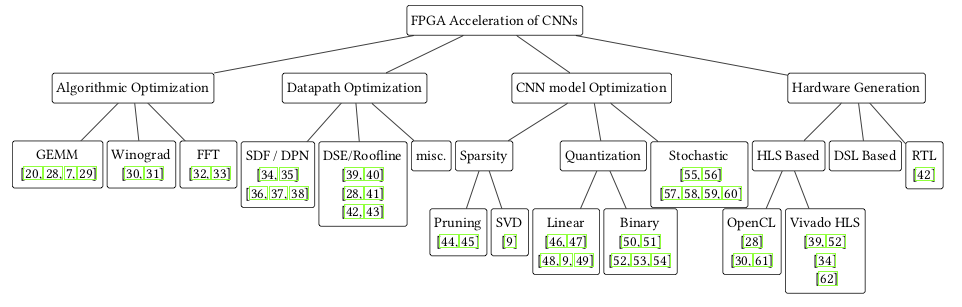
\includegraphics[width=\textwidth]{Figures/InferenceOpt.png}
	\caption[Inference Optimisations]{Methods to accelerate an FPGA implementation \cite{Abdelouahab2018}}
	\label{fig:InferenceOpt}
\end{figure}

The main strategies are:
\begin{itemize}
	\item Algorithmic optimisations: GEMM transformation, Winograd transform, Fast Fourier Transform .
	\item Data-path optimisations: Systolic arrays, SIMD and loop optimisations, Data-flow MoC.
	\item Approximate computations: Fixed-point, Quantisation \cite{Hubara2016}, Dynamic Fixed-point Binary \cite{Courbariaux2016} and Pseudo-Binary nets.
	\item Reduce computations: Weight pruning \cite{Radu2020}, Low rank approximations.
\end{itemize}

Several solutions found in the literature present combination of three strategies to perform best on a given architecture. These works present several ways to tune a CNN to perform best. When looking globally, re-centring to mixed-precision we can see that, as concluded in \cite{Abdelouahab2018}, \guille{CNNs are by nature over-parameterised and support particularly well approximate tuning techniques such as weight pruning and fixed-point computation}.

Quantisation or the use of reduced precision applied to network parameters has been the focus of the literature in the last years. Hubara et al. \cite{Hubara2016} present a way to train a quantised neural network with extremely low precision parameters. The Quantised Neural Networks (QNNs) they train achieve comparable prediction accuracy on well-known datasets such as: MNIST (hand-written digits) \cite{Lecun2010}, CIFAR-10 (tiny images in 10 distinct classes of animals or vehicles) \cite{Krizhevsky2012}, SVHN \cite{Netzer2011} and ImageNet \cite{ImageNet2009}.

An even more agressive vision of quantisation is the use of binary parameters (either +1 or -1). Courbariaux et al. \cite{Courbariaux2016} implemented this type of Binarised Neural Network (BNN) and manage to keep the prediction accuracy for the same above datasets. Both implementations were conducted on GPUs but their FPGA counterpart have been developed later on. Liang et al. \cite{Liang2017} present a BNN implemented on an FPGA and the benchmarked results show an improvement in speed and energy efficiency over other computing platforms.

\subsection{FGPA Frameworks \& Compression Tools}
Improvements on state-of-the-art performance can come from either novel training methods or efficient hardware design. The diversity of FPGAs in terms of designs and manufacturers brought the focus on higher-level tools and frameworks. The field of CNN presents several frameworks to help the design and hardware implementation, automation in the selection of the precision of the parameters and neural network compression tools. They all result in more efficient hardware design and therefore better performance.

FPGAs run against several bottlenecks such as limited bandwidth and on-chip memory. However, due to their flexible nature, CNNs can be adapted to be run on them. Qiu et al. \cite{Qiu2016} show in their state-of-the-art study that the Convolutional layers are computationally-centric and Fully-Connected layers are memory-centric. This means that using any of the two layers will have to bring a concern on the associated bottleneck it holds as well.

Those bottlenecks can be handled automatically using frameworks to generate hardware design and tailor needed precisions. Zhao et al. \cite{Zhao2016} designed F-CNN, the first FPGA framework to train CNNS. Later on, Wang et al. \cite{Wang2018} developed a design flow for extremely low-bit neural networks that focuses on quantisation in both training and FPGA deployment. They aimed at strict resources and power constraints in order to provide a design to the developer. Ding et al. \cite{Ding2019} propose a \guille{Resource-aware, efficient quantisation framework} for object detection on FPGAs. They present an extension and automation of the YOLO model used in the object detection field. Jahanshahi et al. \cite{Jahanshahi2019} present TinyCNN, a modular CNN framework using 16-bit fixed-point data . Zhao et al. \cite{Zhao2019} present Tomato, \guille{a framework designed to automate the process of generating efficient CNN accelerators}. Tomato uses different arithmetics and precisions within each Convolutional layer. This is the first multi-precision multi-arithmetic auto-generation framework for CNNs. fpgaConvNet \cite{Venieris2017} automates the mapping of CNNs on FPGAs using application-level needs (throughput, latency or multiobjective criteria).

Another way to optimise the performance of Neural Networks is the use of compressions. Compressing a neural network results in lowering the precision of its parameters. Tools have been developed to automate the process on several hardware architecture. Distiller is an Intel product built as a Python package on a PyTorch environment. This package focuses more on GPUs. On the other hand, FINN \cite{Umuroglu2017} has been developed as an open-source framework by the FPGA manufacturer Xilinx. It works as a network compression tool especially tailored for FPGAs and have been actively under development with extensions to quantised networks \cite{Blott2018} or Long Short-Term Memory (LSTM) networks \cite{Rybalkin2018}.

\section{Takeaway from the Literature Review}
In this \emph{Literature Review}, the focus went from the backend different number representations and their link to performance to frontend applications that take profit from any gain in energy or time. These applications can be found in different scientific fields such as mathematics, physics simulations and deep learning applications. Different hardware architectures are used to perform the described applications in parallel.

The focus is then put on Convolutional Neural Networks and their application to FPGAs. This choice is made because CNNs have many state-of-the-art application in image recognition, speech recognition or data classification. FPGAs on the other hand offer natural mixed-precision flexible design to build upon. If focus has been put on different types of networks and their associated performance on well-known datasets, very few effort \cite{Bacchus2020} has been put on the quantification of the precision needed and benchmarking. Several articles from the literature often propose an empirical choice in parameters size along with the architecture and performance they got out of the experiment. Bacchus et al. \cite{Bacchus2020} benchmark the trade-offs between training-time, hardware efficiency and accuracy in QNNs while varying the size of the parameters. The work proposed could be extended with new frameworks, architectures and  datasets. The experiment could be reconducted on different architectures and datasets in order to confirm or invalidate the sweet spots found. An extension to Distiller or Brevitas (with PyTorch) could widen the benchmark.
